\section{Simulation Results}
We consider simulating the full Trinity super computer.
The number of compute nodes on Trinity is about 18936, 9436 Intel Haswell nodes
and at least 9500 Intel Xeon Phi nodes.
There are 16 cores on each processor, thus totally 302976 cores.
In the following experiments, we compare two identical system except that
IO nodes are replaced by the same number of burst buffer nodes.
Burst buffer nodes provide total capacity of 4.0 PB PCIe SSD intermediate storage.
Eventually Trinity will support up to 576 burst buffer nodes of 3.7 PB.
Sequential read/write between burst buffer and compute nodes is 8.0 GB/s.
Bandwidth between CPU node and IO node is set to 2.5 GB/s.
Job trace is from ANL's Blue Gene Intrepid system from January to September 2009.
Each log entry contains information like jobs' submission time, running time,
number of cores user requested and so on. 
It is truncated so that only the first 1000 jobs are used in simulation.
We patched 3 fields to each job's log entry: the amount of input data $data\_in$,
the amount of written data during checkpointing $data\_run$ and the amount of output data $data\_out$.
We assume they follows uniform distribution with low boundary 1 TB and high boundary 60 TB.

Following sections discuss or answer 3 key questions.
Will Cerberus improve application performance by utilizing burst buffer nodes?
Can Cerberus with optimization improve application performance?
Will job demand on burst buffer effect Cerberus?

\subsection{Cerberus vs. 1-Phase Batch Scheduler}
\label{Sec:Sim:BBvsIO}
In this section, we demonstrate that by utilizing burst buffer nodes,
job scheduler could improve the applications' performance.
Figure x compares CDF of the response time of 1000 jobs.
When scheduler can allocate burst buffer to jobs,
all jobs finish in 360,000 seconds counting from their submission time.
However, the worst case in system without burst buffer is catastrophical.
There are jobs that takes 1,400,000 seconds to finish,
almost as 4 times slow as the most non-responsive job in system equipped with burst buffer.
In average case, more than 90\% of the jobs scheduled by Cerberus response faster than 1-Phase Batch scheduler.
The improvement mainly comes from the difference of IO operation efficiency between
traditional IO nodes and burst buffer nodes.
There are only less than 10\% of the jobs response quicker without needing burst buffer.



\subsection{Cerberus vs. Cerberus with Optimization}
If we consider optimizing either burst buffer's data throughput or the parallelism across jobs,
dynamic programming based job scheduler can further reduce jobs' wait time.
We plot in Figure x the resulting response time of three different scheduler
regarding how they handle jobs in their queues(input queue, run queue, and output queue).
The first scheduler uses naive first come first serve (FCFS) policy.
Whoever at the front of queue are considered favorably.
The second and third scheduler treat jobs in run queue identically.
They choose jobs according to the optimization solution given by \ref{Equ:MaxProductRecursion}
However, they treat jobs in the input queue and output queue differently.
The second scheduler will select these jobs in its queue so that volume of transferred data is maximized.
The third scheduler tries to optimize the number of schedulable jobs by using \ref{Equ:MaxTaskNumberRecursion}.

\begin{figure}[!t]
\centering
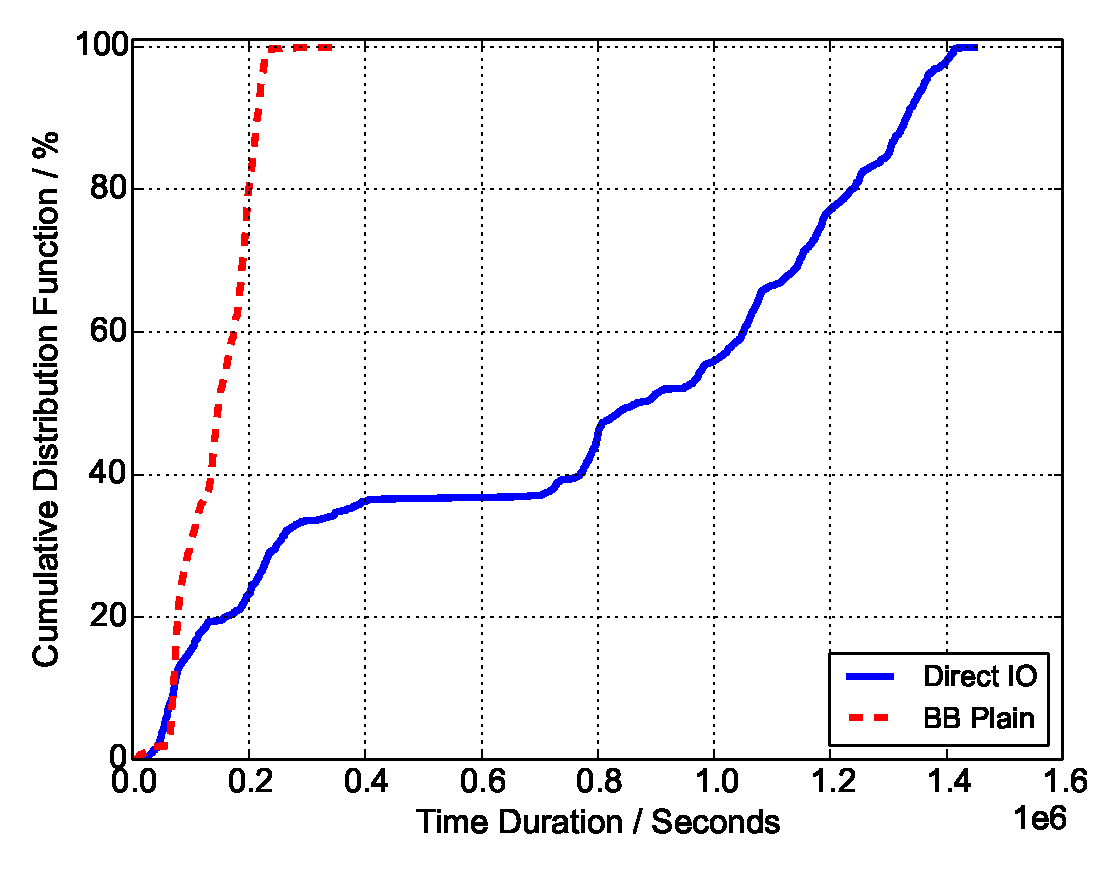
\includegraphics[width=3.2in]{DrawDirectIOvsBB/1000jobs_direct_vs_bb_response}
\caption{Application Response Time, IO Node Only vs. Burst Buffer System}
\label{Fig:DirectIOvsBBResponseTime}
\end{figure}

\begin{figure}[!t]
\centering
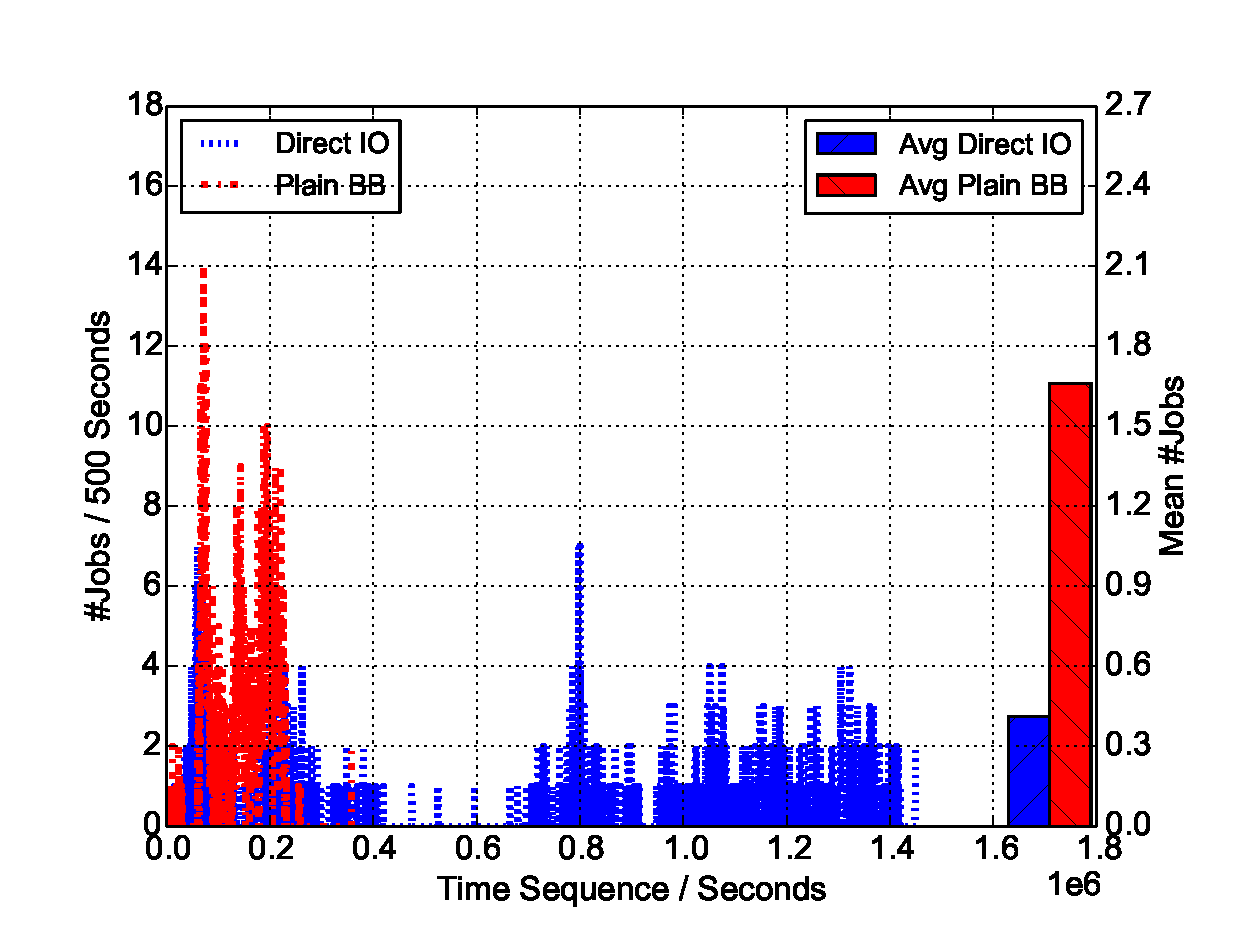
\includegraphics[width=3.2in]{DrawDirectIOvsBB/1000jobs_direct_vs_bb_throughput}
\caption{Application Throughput, IO Node Only vs. Burst Buffer System}
\label{Fig:DirectIOvsBBThroughput}
\end{figure}


\begin{figure}[!t]
\centering
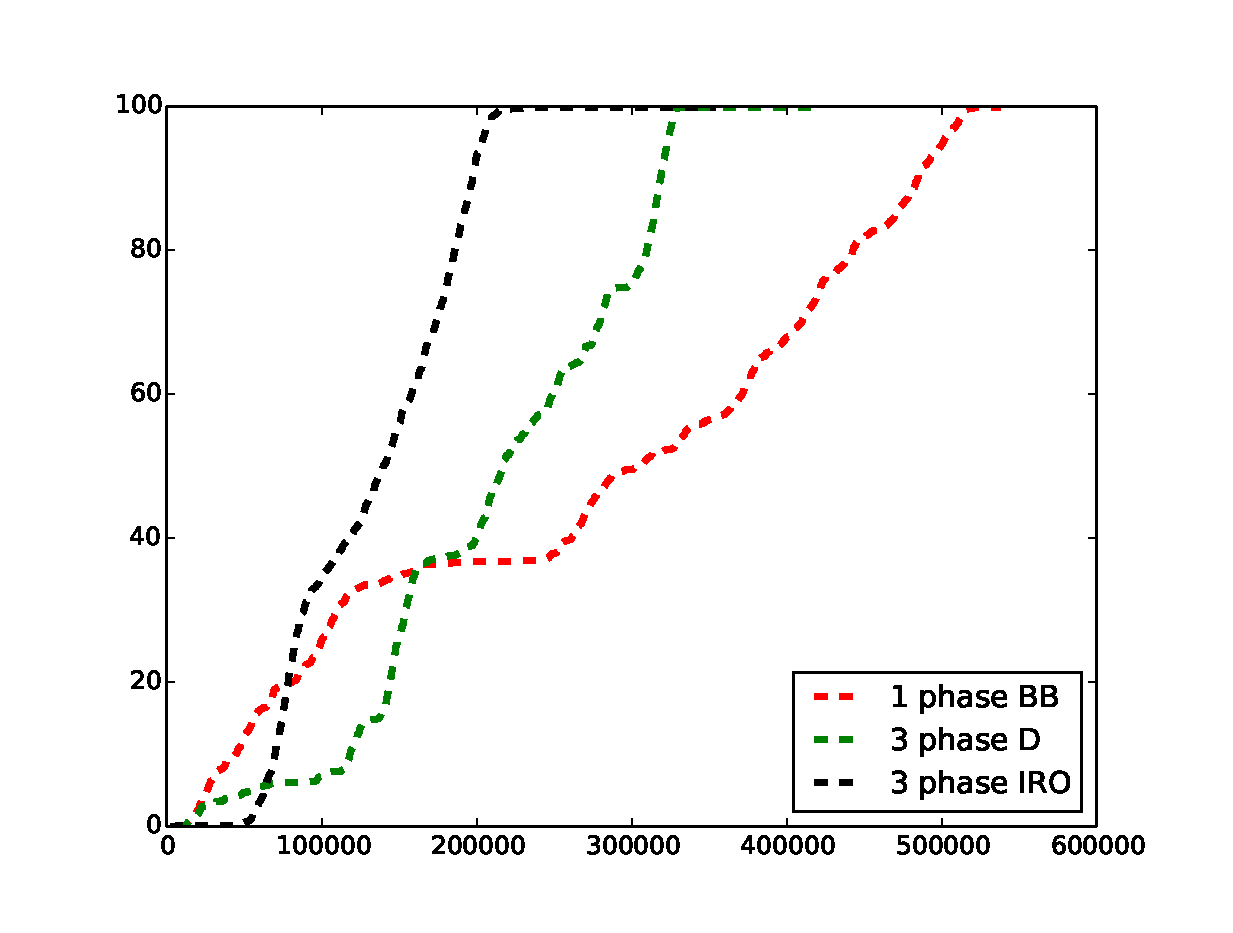
\includegraphics[width=3.2in]{Draw3Pvs1P/1000jobs_3p_vs_1p_response}
\caption{Application Response Time, 1 Phase Model vs. 3 Phase Model}
\label{Fig:3Pvs1PResponseTime}
\end{figure}

\begin{figure*}[!t]
\centering
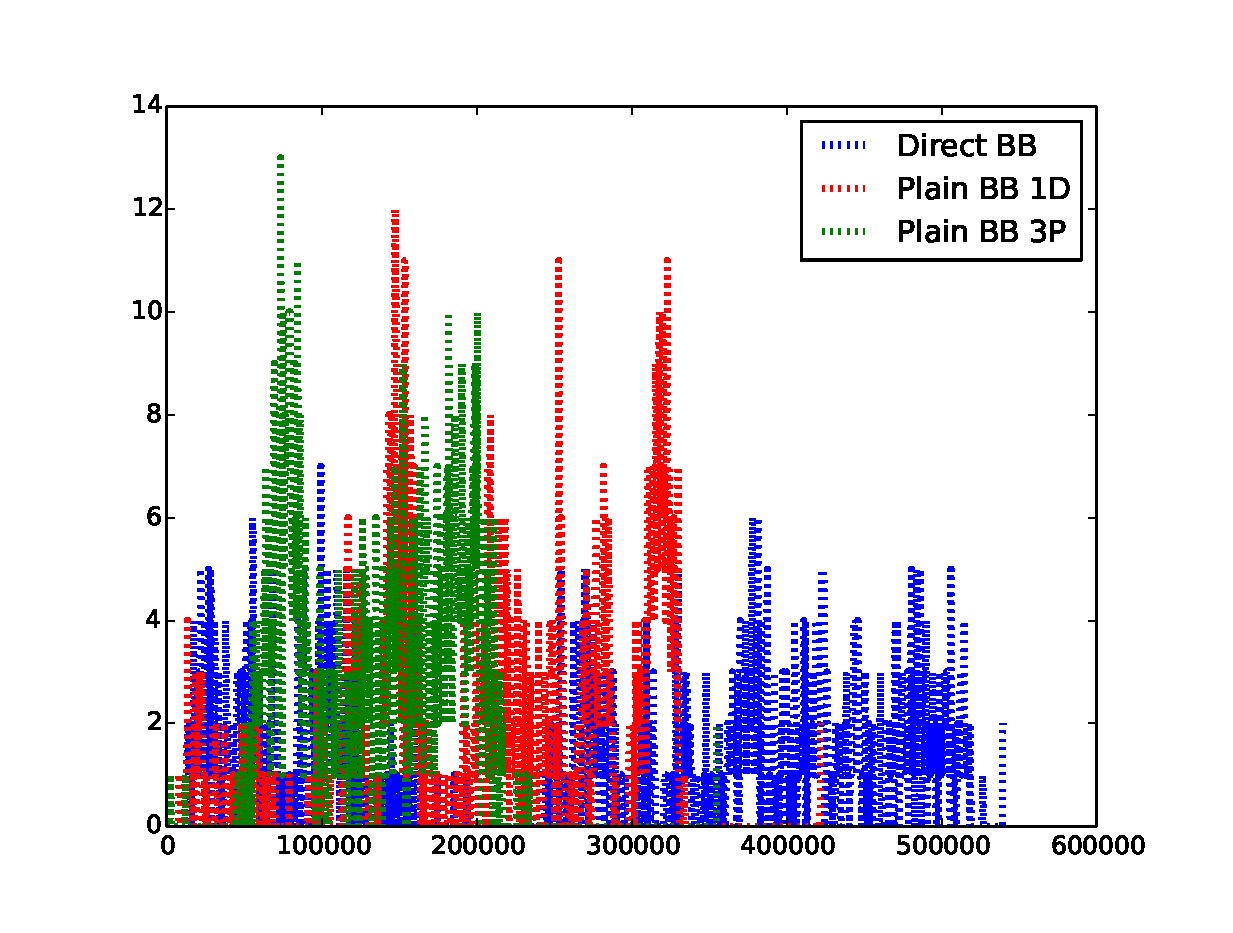
\includegraphics[width=6.2in]{Draw3Pvs1P/1000jobs_3p_vs_1p_throughput}
\caption{System Throughput, 1 Phase Model vs. 3 Phase Model}
\label{Fig:3Pvs1PThroughput}
\end{figure*}


\subsection{Cerberus vs. Demand Granularity}
In this section we validate our 3-phase model.
Applications are benefited when scheduler dividing jobs into 3 separated phases and 
scheduling are based on corresponding burst buffer demand in each phase.
This suggests that user should provide burst buffer demand as granular as possible.

In Figure \ref{Fig:3Pvs1PResponseTime}, we plot 3 different scheduling results by 3 FCFS scheduler.
Jobs in the first case, denoted as 1 phase BB, are modeled as just 1 phase because user just provides
a general burst buffer demand throughout entire application life time.
We assume this demand is the $\max \{data\_in, data\_out, data\_run\}$.
This is the traditional scheduling scheme except job has additional
burst buffer demand and scheduler must subject to burst buffer capacity constraint.
Jobs in the second and third cases have 3 phases and are scheduled by Cerberus.
However, in the second case, denoted as 3-phase D, Cerberus only knows the overall burst buffer demand,
same as the information in case 1.
In the 3rd case, named 3-phase IRO, users kindly provided all the burst buffer demand in all 3 phases.
This is the same case as in section \ref{BBvsIO} when we demonstrating burst buffer is beneficial.
We simulate the 3 cases with the same generated random data volume.
For 1-phase-modeled jobs, scheduler will make decision based on $\max \{data\_in, data\_out, data\_run\}$
since we assume user will only tell the upper bound of its application's demand.
However, in simulation, we use the generated data amount as the same as 3-modeled jobs.
%Response time of system without burst buffer devices are also plotted for comparison.

Unsurprisingly, jobs' response time is improving as long as they could utilizing burst buffer.
Let's compare scheduling results of 1-phase and 3-phase, both of which only have rough data information of application.
More than 60\% of the 3-phase-modeled jobs finish faster than 1-phase-modeled jobs.
The longest 3-phase-modeled job takes 400,000 seconds to finish while the slowest 1-phase-modeled job
needs about 540,000 seconds to finish.
The improvement is about 26\% for the worst case.
The reason of such improvement is as follows.
For the 1-phase-modeled jobs, burst buffer nodes will be exclusively taken by scheduled jobs
throughout their lifetime.
In contrast, each time a 3-phase-modeled job finish inputing, running or outputing,
Cerberus will reclaim burst buffer and CPU resources.
This gives Cerberus more opportunity to schedule the system resources.
At last, when comparing the case of 3-phase IRO with 3-phase D, we find another advantage of our 3-phase model.
If benign users can provide finer-grain information of data/IO demand,
Cerberus can programme each queue separately and get better scheduling result.
In our simulation, when Cerberus knows more about application's demand in different phases,
the worst absolute response time is less than 300,000 seconds.
This is 25\% improvement to 3-phase-modeled jobs when Cerberus only knows the upper bound of data demand,
44\% better than the slowest 1-phase-modeled job.
In average case, 80\% of the 3-phase-modeled jobs scheduled by Cerberus finish earlier than 1-phase-modeled jobs,
on the same condition that the same amount of burst buffer nodes are available to applications.
Meanwhile, more than 90\% of the jobs takes less time if user specifies data usage demand
at each phase to Cerberus.

Figure x describes system throughput of these three different scenarios.
It helps us examine the performance of the scheduling in time sequence.
For 1-phase-modeled job, we can see an obvious 'throughput gap'
from 150,000 second to 250,000 second approximately.
This is the result of too aggressive scheduling at the beginning.
For the case of 3-phase D, throughput also starts provocatively,
but not as provocatively as 1-phase scheduling case;
it is then calmed due to frequent resource release,
indicated by multiple crests and troughs from 0 to 350,000 seconds.
The 3-phase IRO runs counter to the both previous cases.
Even though beginning with throughput trough,
Cerberus manages to make the system having high throughput from 50,000 to 250,000 seconds,
during which system can achieve throughput around 10 to 12 per 500 seconds. 



